\documentclass[../main.tex]{subfiles}
\graphicspath{{\subfix{../figures/}}}
%
\begin{document}
\section{状态模式(State)}
状态模式,又称状态对象模式。状态模式是对象的行为模式[GOF95]
状态模式允许一个对象在其内部状态改变的时候改变其行为。这个对象看上去就像是改变了它所属的类一样。

很多情况下,一个对象的行为取决于一个或多个动态变化的属性,这样的属性叫做状态,这样的对象叫做有状态的对象。
这样的对象状态通常是从一系列预定义的值中取出的。
%
\begin{lstlisting}[language=java]
class Elevator {
  int level; //-2表示最底层
  int state; //1表示正常,2表示故障,3表示检修
  void onDownButtonPressed() {
    if(level==-2 || state!=1) {
      //do nothing
    } else {
      //电梯向下
    }
  }
}
\end{lstlisting}
%
\subsection{状态模式的结构}
状态模式把对象的行为包装在不同的状态对象里,状态对象都属于一个抽象状态类的一个子类。状态模式的意图是让一个对象在其内部状态改变的时候,其行为也随之改变。状态模式的示意性类图如下:
%
\begin{figure}[H]
  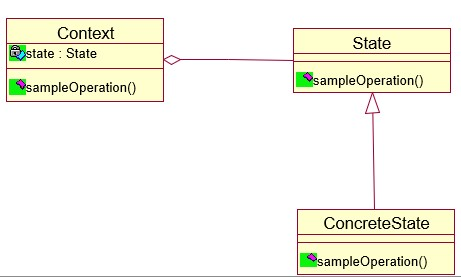
\includegraphics[width=0.55\textwidth]{31_1.jpg}
\end{figure}
%
\textbf{模式所涉及的角色有}:
\begin{itemize}
  \item 抽象状态角色:定义一个接口,用以封装环境(Context)对象的一个特定的状态所对应的行为。
  \item 具体状态角色:每一个具体状态类都实现了环境(Context)的一个状态所对应的行为。
  \item 环境角色:定义行为将随状态变化的对象,并持有一个具体状态对象的引用。
\end{itemize}
%
下面是环境角色Context的源代码,可以看出,环境类持有一个State对象,并把所有的行为委派给此对象。
%
\lstinputlisting[language=java]{./code/31/1/Context.java}
\lstinputlisting[language=java]{./code/31/1/State.java}
\lstinputlisting[language=java]{./code/31/1/ConcreteState.java}
%
\subsection{使用场景}
在以下各种情况下可以使用状态模式:
%
\begin{enumerate}
  \item 一个对象的行为依赖于它所处的状态,对象的行为必须随着其状态的改变而改变。
  \item 对象在某个方法里依赖于一重或多重的条件转移语句,其中有大量的代码。状态模式把条件转移语句的每一个分支都包装到一个单独的类里。这使得这些条件转移分支能够以类的方式独立存在和演化。
\end{enumerate}
%
\subsection{例:TCP}
考虑由TcpConnection代表一个TCP/IP网络的连接。
一个TcpConnection对象可以具有以下状态之一:Listening(监听)、Established(已建立连接)、Closed(关闭)。当TcpConnection对象接到其它对象的请求时,会根据其状态不同而给出不同的回应。TCP系统的UML类图如下所示:
%
\begin{figure}[H]
  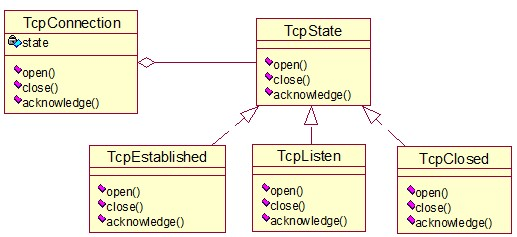
\includegraphics[width=0.55\textwidth]{31_2.jpg}
\end{figure}
%
在此,使用状态模式的关键是引进了抽象类或接口TcpState来代表网络的连接状态。它的子类实现了由状态决定的行为。
TcpConnection类持有一个状态对象,TcpState子类的实例,来表示TCP连接的现在状态。 TcpConnection类把所有与状态有关的请求都委派给它的状态对象。 TcpConnection使用它的TcpState的子类实例来执行特定的连接状态所对应的操作。
当连接的状态改变时, TcpConnection对象就改变它所用的状态对象。例如,当网络连接从“已建立"改为“关闭"时, TcpConnection对象会把它的状态对象从TcpEstablished的实例改为TcpClosed的实例。

\textbf{系统有如下的角色}:
%
\begin{itemize}
  \item 环境角色:TcpConnection。此类定义了客户端感兴趣的接口,并持有有关具体状态类的实例,以定义它当前所处的状态。
  \item 状态角色:TcpState。此类定义了把依赖于一个特定的状态所对应的行为包装起来所需要的接口。
  \item 具体状态角色:TcpEstablished、TcpListen、TcpClosed。实现了环境类的状态所对应的行为。
\end{itemize}
%
\lstinputlisting[language=java]{./code/31/2/TcpConnection.java}
\lstinputlisting[language=java]{./code/31/2/TcpState.java}
\lstinputlisting[language=java]{./code/31/2/TcpEstablished.java}
%
\subsection{例:用户登录子系统}
用户进入系统时首先遇到登录页面,输入用户名和密码,单击〔log on〕键,系统会向数据库查询。登录成功后,就会见到欢迎页面。登录失败,仍然要面对登录页面。下图描述了用户的状态变化情况。
%
\begin{figure}[H]
  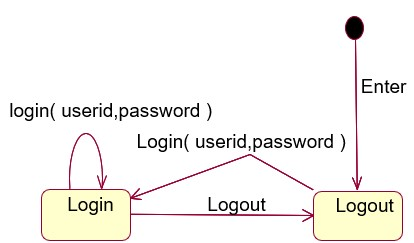
\includegraphics[width=0.45\textwidth]{31_3.jpg}
\end{figure}
%
从上面的状态图可以看出,用户进入系统时,处于Logout状态,用户输入正确的用户名和密码可以过渡到Login状态。当用户处于Login状态时,可以发出Logout命令,使系统过渡到Logout状态。用户在Login状态时,重新发出Login的命令不会改变状态。

不同的状态会产生不同的网页,对应于Login状态的是欢迎页面,对应于Logout状态的是登录页面。登录页面提交后的Servlet是ContextServlet。这个servlet在doGet或doPost方法中接收用户名和密码,并且创立对应的状态对象。
%
\begin{figure}[H]
  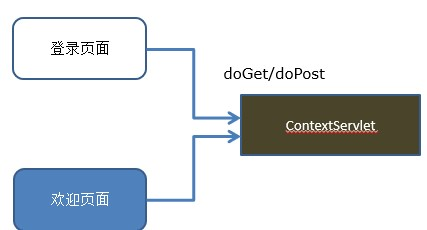
\includegraphics[width=0.40\textwidth]{31_4.jpg}
\end{figure}
%
登录子系统的静态结构图如下:
%
\begin{figure}[H]
  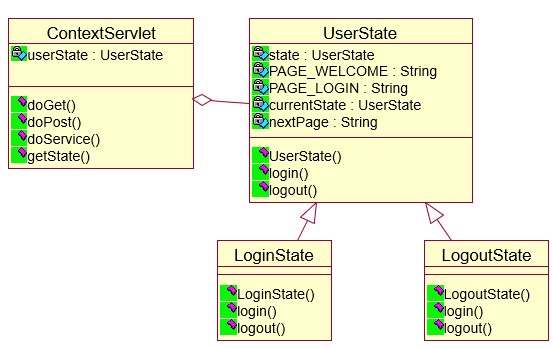
\includegraphics[width=0.50\textwidth]{31_5.jpg}
\end{figure}
%
登录页面的源代码如下:
%
\begin{lstlisting}[language=html]
<HTML>
  <BODY>
     <FORM action=“/Servlet/com.javapatterns.state.login.ContextServlet"
    method=get>
   User ID<INPUT TYPE=text name=userid value=“jeff"><br>
   Password < INPUT TYPE=password name=password    value=“pass"><br>
      <input type=submit name=“btnAction" value=“Log On">
     </FORM>
   </BODY>
</HTML>
\end{lstlisting}
%
登录后的页面(欢迎页面)。其源代码如下:
%
\begin{lstlisting}[language=html]
<HTML>
  <BODY>
     <FORM action=“/Servlet/com.javapatterns.state.login.ContextServlet"
    method=get>
   Welcome to website!<br>
      <input type=submit name=“btnAction" value=“Log Out">
     </form>
   </body>
</html>
\end{lstlisting}
%
环境类ContextServlet的源代码如下:
%
\lstinputlisting[language=java]{./code/31/3/ContextServlet.java}
%
环境类首先判断客户端的请求是登录还是退出。当接到登录请求时,环境类调用状态类的login()方法。当接到退出请求时,环境类调用状态类的logout()方法。

抽象类UserState代码清单如下:
%
\lstinputlisting[language=java]{./code/31/3/UserState.java}
%
子系统的具体类LoginState包装了系统在登录成功后的Login状态。其源代码如下:
%
\lstinputlisting[language=java]{./code/31/3/LoginState.java}
%
子系统的具体类LogoutState包装了系统在登录失败后的Logout状态。其源代码如下:
%
\lstinputlisting[language=java]{./code/31/3/LogoutState.java}
%
\end{document}
